\documentclass[a4paper,11pt]{article}
\usepackage[utf8]{inputenc}
\usepackage{amsmath}
\usepackage{amsfonts}
\usepackage{amssymb}
\usepackage{graphicx}
\usepackage{braket}
\usepackage{listings}

\numberwithin{equation}{section}
\renewcommand\thesubsection{\alph{subsection}}
\newcommand{\bvp}[1]{\mathbf{#1}'}
\newcommand{\bv}[1]{\mathbf{#1}}

\lstset{breaklines=true}

%opening
\title{Computational Biophysics HW2}
\author{Vince Baker}

\begin{document}

\maketitle

\section{Q1}
Speed: computational complexity is a critical factor computational science, but for computational biology the numerical integration is not the complexity driver.
The force calculations required for many-body molecular dynamics take far more computational time than the numerical integration itself. 
To minimize the required computational complexity one should choose the numerical integration method that requires the fewest acceleration updates.\\
Closeness to classical trajectories: Many-body dynamical systems are chaotic, so small errors in a particle's state will cause the phase space trajectory to rapidly diverge from the classical trajectory.
This is generally unimportant since computational biophysics investigates the larger-scale properties of systems, not the specific trajectories of individual molecules.\\
Conservation laws: Molecular dynamics simulations should obey the appropriate conservation laws. 
Significant (unexpected) fluctuations in energy or momentum indicate non-physical behavior, and indicate that the time step should be reduced or a different integration algorithm should be chosen.\\
Time reversibility: Similar to the deviation from classical trajectories, molecular dynamics simulations will not generally be time-reversible due to the chaotic nature of many-body systems.
\\
\section{Q2}
Assuming the system being simulated is not a crystal, the random particle positions are more representative of a physical state of the system.
However, a system that starts in a lattice will quickly become randomized during the simulation. 
Lattice placement is faster but will require a number of simulation steps for the system to randomize, during which data collected from the system is not valid.
Random placement gives a more realistic initial system but the initialization takes longer, and it's possible to specify a set of conditions that will result in the random placement routine running indefinitely.
\\
\section{Q3}
The pair correlation function of a crystal will have extremely strong, narrow peaks at the multiples of the crystal element spacing.
The pair correlation funciton of a liquid will still have peaks near multiples of the inter-atomic distance due to nearest-neighbor caging, but the peaks will not be as sharp as a crystal.
\section{Q4}
The velocty autocorrelation function is dominated by the strong correlation near $\tau =0$, so the time step and correlation length must be chosen carefully to accurately estimate the transport coefficient.
Measuring the transport coefficient as the slope of the mean-squared displacement over time should be less sensitive to simulation parameters since the line slope measurement naturally incorporates substantial averaging.

\section{P1}
The line of code is at ensemble.cc:354. The mean velocity is calculated during random assignment and then removed by:\\
\begin{lstlisting}
atoms[i].v = ( atoms[i].v - vel_cm ) * fs; 
\end{lstlisting}

\section{P2}
The boundary conditions are implemented by calculating distances using the IMAGE macro starting at forces.cc:72.\\
\begin{lstlisting}
// USE IMAGE DISTANCES\\
dr.x = IMAGE(dr.x, sys.inv_Lx, sys.Lx);\\
dr.y = IMAGE(dr.y, sys.inv_Ly, sys.Ly);\\
dr.z = IMAGE(dr.z, sys.inv_Lz, sys.Lz);\\
\end{lstlisting}
The IMAGE macro itself is defined starting at macros.h:51.\\
\begin{lstlisting}
// -- MINIMUM IMAGE DISTANCE MACRO\\
#define IMAGE(r, boxinv, box) ( (r) - ANINT( (r) * (boxinv) ) * (box) )\\ 
\end{lstlisting}
The ANINT macro rounds a floating-point number to an integer, since the images are exactly one box length from the actual particles.

\section{P3}
The initial and final speed distributions in 2D are plotted in Figure \ref{fig:energyplot}.
The system has clearly relaxed toward the Maxwell-Boltzmann distribution (blue line).
\begin{figure}[h]
 \caption{Initial and final speed distributions}
 \centering
   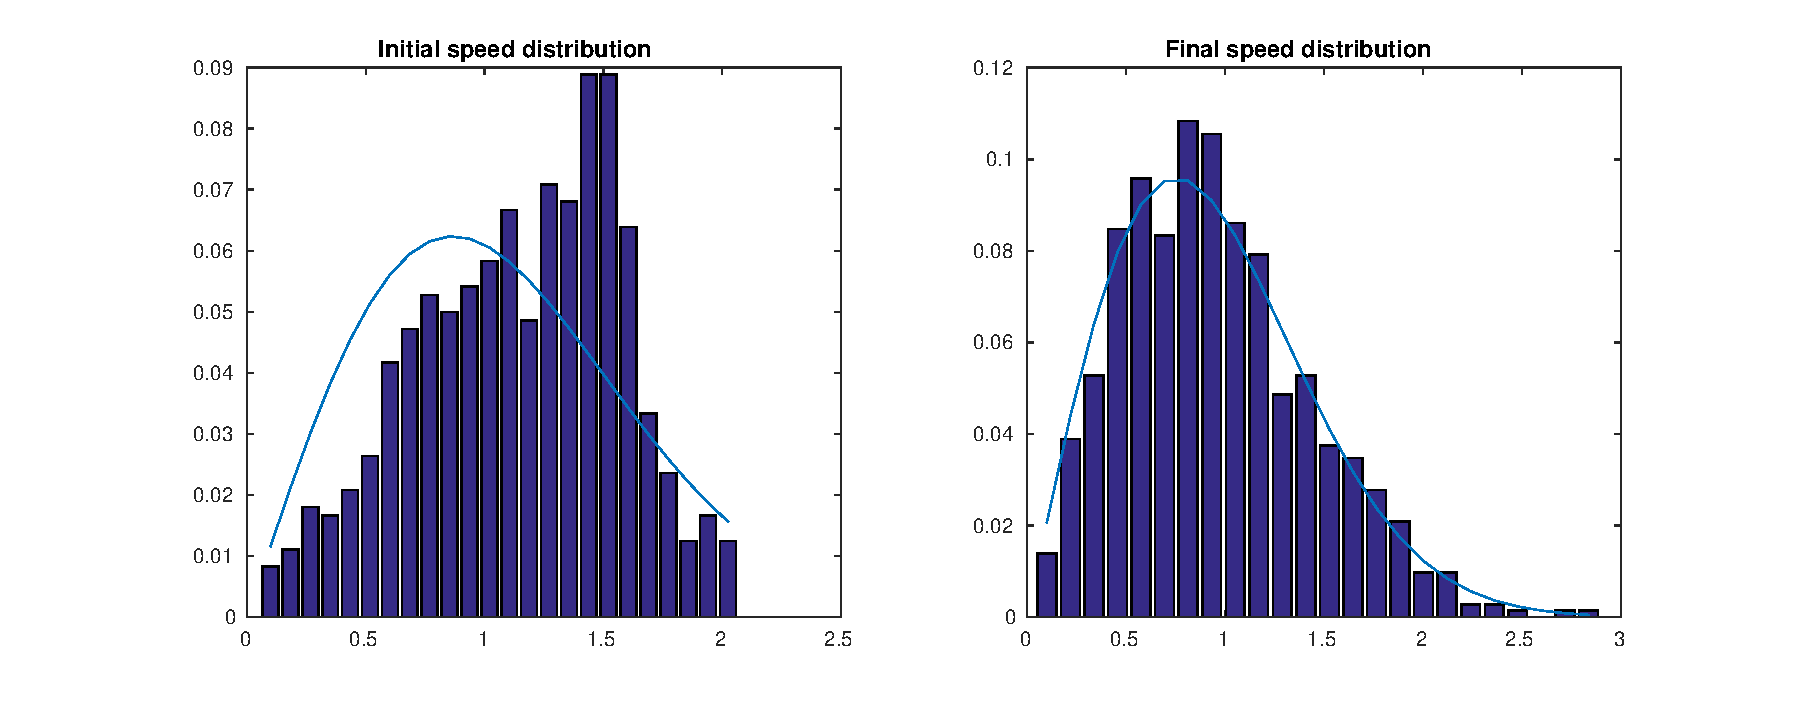
\includegraphics[width=\textwidth]{SpeedDist2D}
 \label{fig:energyplot}
\end{figure}
\\
The 3D plots show similar behavior in the 3D system.
\begin{figure}[h]
 \caption{Initial and final speed distributions (3D)}
 \centering
   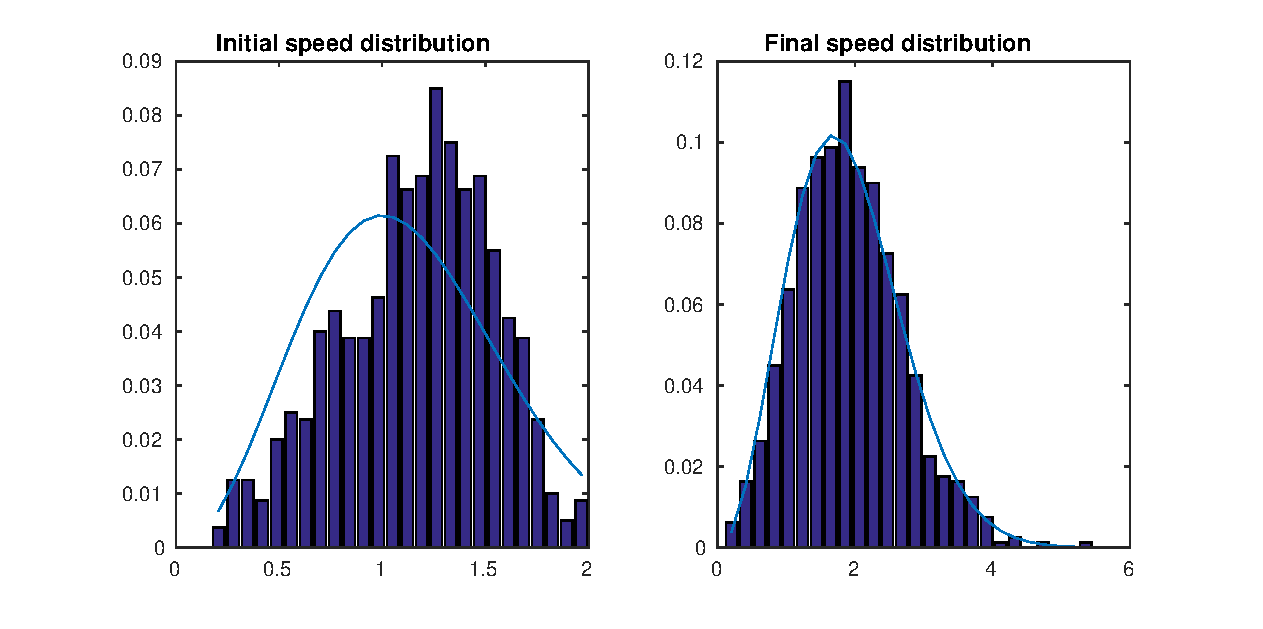
\includegraphics[width=\textwidth]{SpeedDist3D}
 \label{fig:energyplot3d}
\end{figure}

\section{P4}
The figure below shows a Gaussian distribution (middle) derived from samples from a uniform distribution (left).
The figure on the right is the Gaussian distribution shifted and scaled to $\mu =3$, $\sigma=0.5$.
\begin{figure}[h]
 \caption{Gaussian distribution derived from samples from uniform distribution}
 \centering
   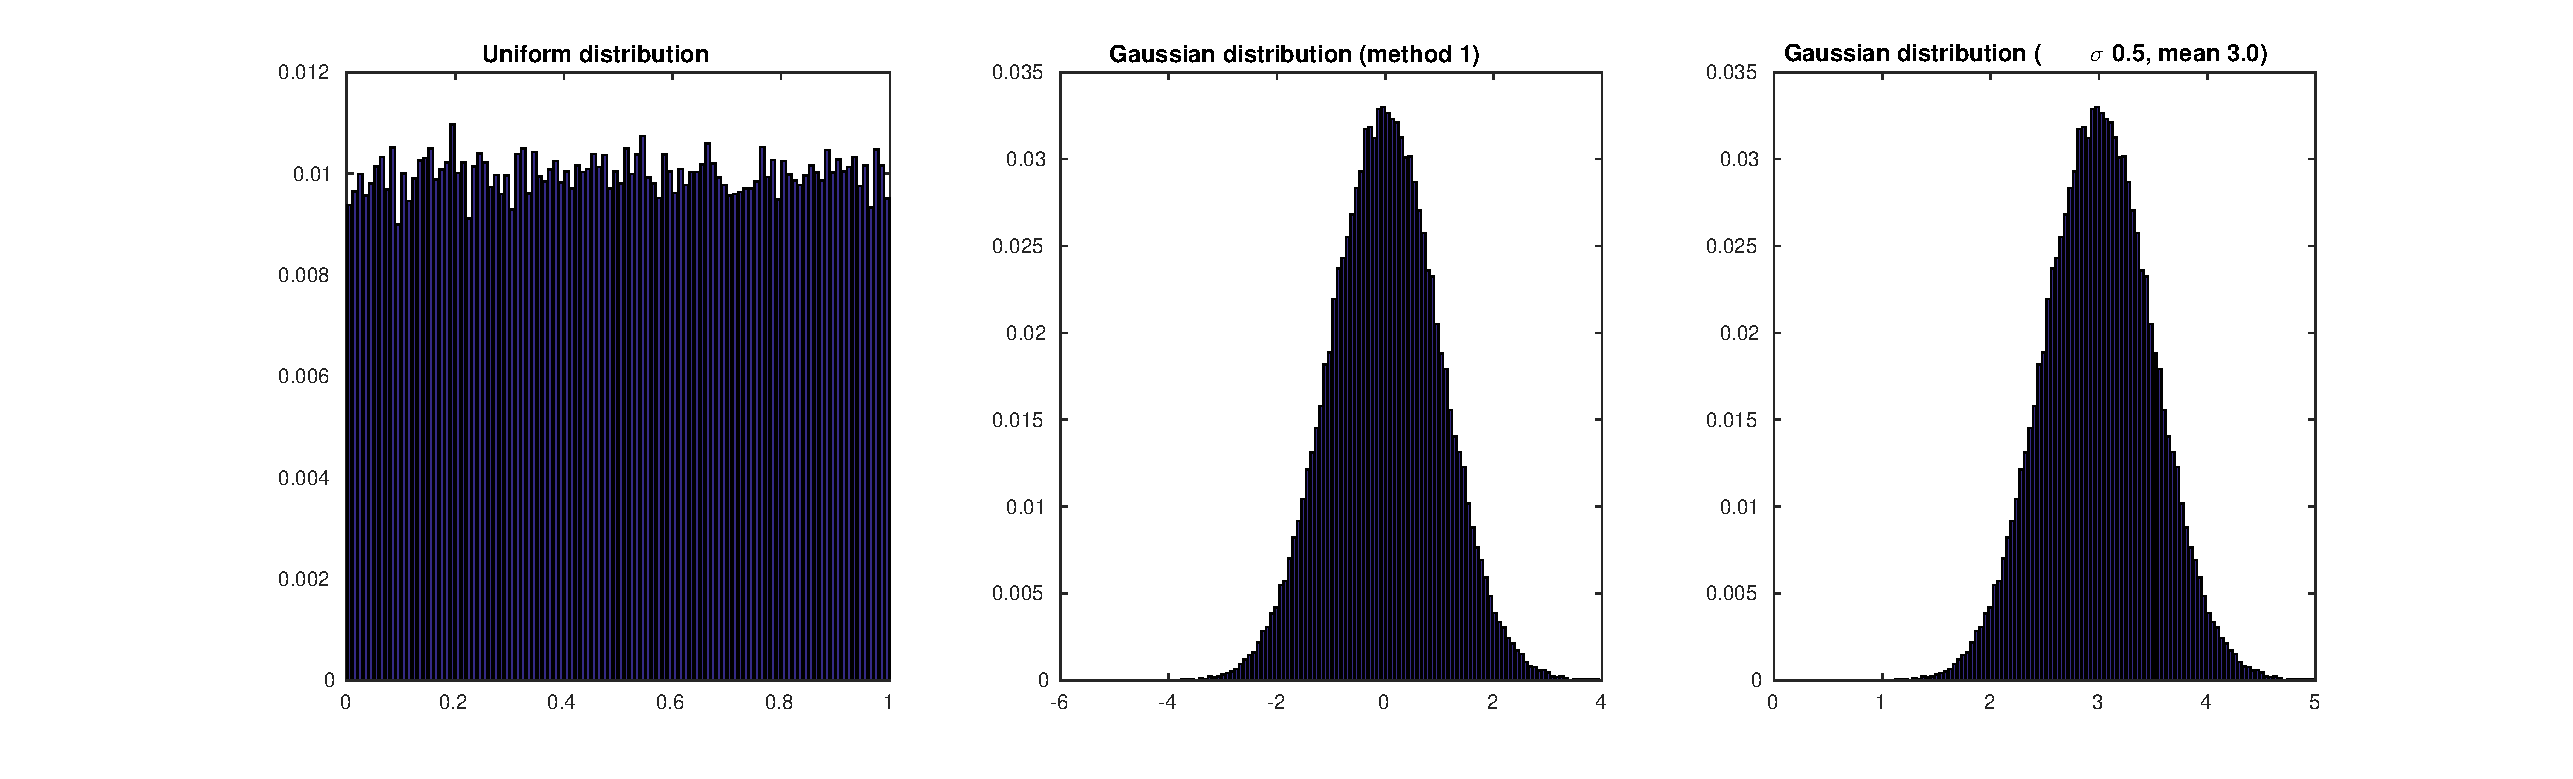
\includegraphics[width=\textwidth]{p4_distributions}
\end{figure}

\section{P5}
The results of the Guassian generation algorithm for different values of N is plotted below.
The algorithm with N=12 clearly agrees best with the actual Gaussian (solid red line).
\begin{figure}[h]
 \caption{Approximations to Gaussian distribution}
 \centering
   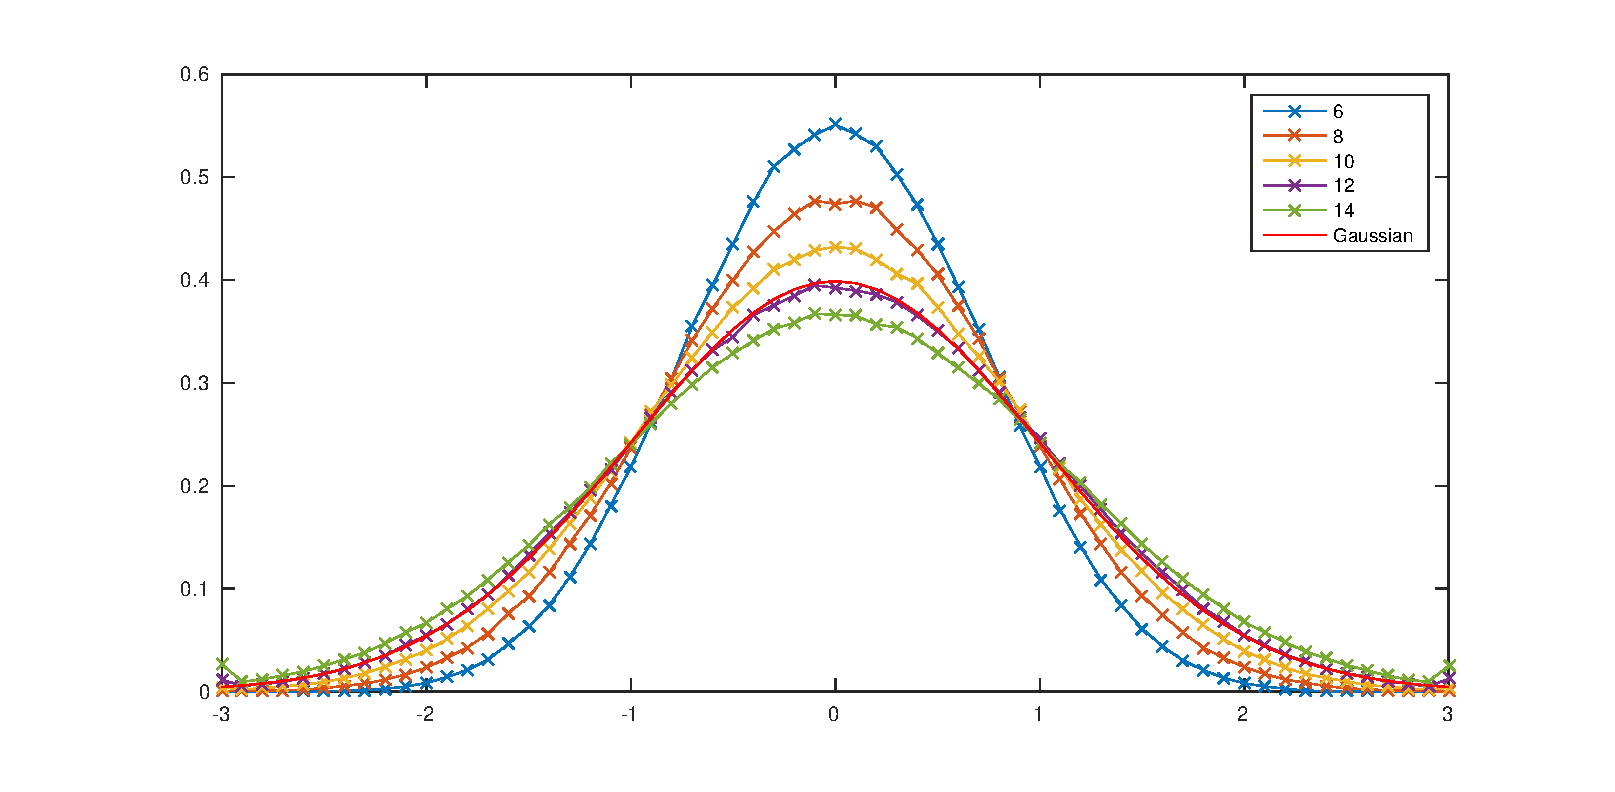
\includegraphics[width=\textwidth]{p5_gaussians}
\end{figure}

\end{document}
